\documentclass{article}
\usepackage[utf8]{inputenc}
\usepackage{t1enc}
\usepackage{geometry}
 \geometry{
 a4paper,
 total={210mm,297mm},
 left=20mm,
 right=20mm,
 top=20mm,
 bottom=20mm,
 }
\usepackage{amsmath}
\usepackage{amssymb}
\usepackage{pgf,tikz}
\usetikzlibrary{arrows}
\frenchspacing
\usepackage{fancyhdr}
\pagestyle{fancy}
\lhead{Urbán János tanár úr feladatsorai}
\chead{C08/08/1. csoport}
\rhead{Egyenlőtlenségek}
\lfoot{}
\cfoot{\thepage}
\rfoot{}

\usepackage{enumitem}
\usepackage{multicol}
\usepackage{calc}
\newenvironment{abc}{\begin{enumerate}[label=\textit{\alph*})]}{\end{enumerate}}
\newenvironment{abc2}{\begin{enumerate}[label=\textit{\alph*})]\begin{multicols}{2}}{\end{multicols}\end{enumerate}}
\newenvironment{abc3}{\begin{enumerate}[label=\textit{\alph*})]\begin{multicols}{3}}{\end{multicols}\end{enumerate}}
\newenvironment{abc4}{\begin{enumerate}[label=\textit{\alph*})]\begin{multicols}{4}}{\end{multicols}\end{enumerate}}
\newenvironment{abcn}[1]{\begin{enumerate}[label=\textit{\alph*})]\begin{multicols}{#1}}{\end{multicols}\end{enumerate}}
\setlist[enumerate,1]{listparindent=\labelwidth+\labelsep}

\newcommand{\degre}{\ensuremath{^\circ}}
\newcommand{\tg}{\mathop{\mathrm{tg}}\nolimits}
\newcommand{\ctg}{\mathop{\mathrm{ctg}}\nolimits}
\newcommand{\arc}{\mathop{\mathrm{arc}}\nolimits}
\renewcommand{\arcsin}{\arc\sin}
\renewcommand{\arccos}{\arc\cos}
\newcommand{\arctg}{\arc\tg}
\newcommand{\arcctg}{\arc\ctg}

\parskip 8pt
\begin{document}

\section*{Egyenlőtlenségek}

\subsection*{2010.01.19. -- Függvények}
\begin{enumerate}
\item Igazoljuk, hogy ha $a,b \ge 0$, akkor  $$\sqrt{ab}\le \dfrac{a+b}{2}$$
és egyenlőség csak akkor teljesül, ha $a=b$.
\item Igazoljuk, hogy ha $a,b > 0$, akkor  $$\frac{2}{\dfrac{1}{a}+\dfrac{1}{b}}\le \sqrt{ab},$$
(a \underline{harmonikus közép} nem nagyobb, mint a \underline{mértani közép}),
egyenlőség csak akkor igaz, ha $a=b$.
\item Igazoljuk a következő egyenlőtlenségeket:
\begin{abc}
\item ha $x,y>0$ és $x+y=1$, akkor $xy\le\dfrac{1}{4}$;
\item ha $a>0$, akkor $a+\dfrac{1}{a}\ge 2$;
\item $(a+b)(b+c)(c+a)\ge 8abc$, ha $a,b,c\ge 0$;
\item ha $a,b\ge 0$, akkor $\dfrac{a+b}{2}\le \sqrt{\dfrac{a^2+b^2}{2}}$.
\end{abc}
\end{enumerate}

\subsection*{2010.01.20.}
\begin{enumerate}
\item Ábrázoljuk a következő függvényeket:
\begin{abc2}
\item $x\mapsto \sqrt{x+2\sqrt{x-1}}, \quad x\ge 1$;
\item $x\mapsto \sqrt{x-2\sqrt{x-1}}, \quad x\ge 1$;
\item $x\mapsto \sqrt{x+2\sqrt{x-1}}+\sqrt{x-2\sqrt{x-1}}, \quad x\ge 1$.
\end{abc2}
\item Oldjuk meg függvények segítségével:
\begin{abc2}
\item $\sqrt{x-2\sqrt{x-1}}+\sqrt{x+2\sqrt{x-1}}=\dfrac{1}{x-1}$;
\item $\sqrt{1-x^2}\ge x$.
\end{abc2}
\item Vázoljuk a következő függvények grafikonját:
\begin{abc3}
\item $x\mapsto x+\dfrac{1}{x},\quad x\ne 0$;
\item $x\mapsto \dfrac{2x}{1+x^2}$;
\item $x\mapsto \sqrt{4-x^2},\quad -2\le x\le 2$.
\end{abc3}

\item ($*$) Igazoljuk, hogy ha $x,y>0$ és $x+y=1$, akkor
$$\left(x+\dfrac{1}{x}\right)^2+\left(y+\dfrac{1}{y}\right)^2\ge \dfrac{25}{2}.$$ 

\end{enumerate}

\subsection*{2010.01.21.}
\begin{enumerate}
\item A következő két szám közül melyik a nagyobb:
$$\sqrt{2009}+\sqrt{2011}\qquad \text{~vagy~}\qquad 2\sqrt{2010}?$$
\item Egy szakasz felé két négyzetet rajzoltunk. Mikor lesz a legkisebb a két négyzet együttes területe?

\item Igazoljuk, hogy ha $a,b,c,d \ge 0$, akkor
$$\sqrt[4]{abcd}\le\dfrac{a+b+c+d}{4}.$$
\item Az előző feladat felhasználásával igazoljuk, hogy ha $a,b,c \ge 0$, akkor
$$\sqrt[3]{abc}\le\dfrac{a+b+c}{3}.$$
\item Egy $a$ oldalú négyzet négy sarkából vágjunk ki egybevágó négyzeteket úgy,
hogy a kapott lap négy szélének felhajtásával keletkező doboz térfogata maximális legyen.
\end{enumerate}

\subsection*{2010.02.02.}
\begin{enumerate}
\item Határozzuk meg a következő függvények legkisebb értékét:
\begin{abc3}
\item $x\mapsto x^2+2x-3, x\in\mathbb{R}$;
\item $x\mapsto 3-x+2x^2, x\in\mathbb{R}$;
\item $x\mapsto x^2+x+5, x\in\mathbb{R}$.
\end{abc3}
\item Határozzuk meg a következő függvények legnagyobb értékét:
\begin{abc3}
\item $x\mapsto x^2-2x-1$;
\item $x\mapsto 1+3x-x^2$;
\item $x\mapsto -2x^2+x+3$.
\end{abc3}

\item Egy adott $a>0$ számot bontsunk fel két pozitív szám összegére úgy,
hogy a kapott részek négyzetének összege a legkisebb legyen.
\item Egy folyó partján egy téglalap alakú területet kell elkeríteni
egy kerítéssel, amelynek kerülete 100~m. Mekkora az a maximális terület, amit így el lehet keríteni?
\end{enumerate}

\subsection*{2010.02.03.}
\begin{enumerate}
\item Igazoljuk, hogy ha $a,b,c>0$ valós számok, akkor
$$\dfrac{3}{\dfrac{1}{a}+\dfrac{1}{b}+\dfrac{1}{c}}\le \sqrt[3]{abc}$$
és az $=$ csak akkor igaz, ha $a=b=c$.
\item Igazoljuk, hogy ha $a,b,c>0$ valós számok, akkor
$$\dfrac{1}{a}+\dfrac{1}{b}+\dfrac{1}{c}\ge \dfrac{9}{a+b+c}.$$
\item Igazoljuk, hogy ha $a_1, b_1,a_2,b_2$ tetszőleges valós számok, akkor
$$a_1b_1+a_2b_2\le \sqrt{a_1^2+a_2^2}\cdot \sqrt{b_1^2+b_2^2}.$$
\item ($*$) Igazoljuk, hogy ha $a\ge b> 0$, akkor 
$$0\le \dfrac{a+b}{2}-\sqrt{ab}\le \dfrac{(a-b)^2}{8b}.$$
\item \underline{Rendezési tétel}: Ha $a\le b \le c$ és $x\le y \le z$ adott számok, akkor 
\begin{align*}
ax+by+cz&\ge ay+bz+cx\ge az+by+cx;\cr
ax+by+cz&\ge az+bx+cy\ge az+by+cx.
\end{align*}
Igazoljuk!
\item ($*$) Bizonyítsuk be, hogy ha $a,b,c>0$ adott számok, akkor
$$\dfrac{a}{b+c}+\dfrac{b}{c+a}+\dfrac{c}{a+b}\ge \dfrac{3}{2}.$$
\end{enumerate}

\subsection*{2010.02.04.}
\begin{enumerate}
\item Oldjuk meg a nemnegatív egész számok halmazán:
$$x\sqrt{1-y^2}+y\sqrt{2-z^2}+z\sqrt{3-x^2}=3.$$
\item Igazoljuk, hogy ha $a,b,c>0$, akkor 
$$a+b+c\le\dfrac{bc}{a}+\dfrac{ac}{b}+\dfrac{ab}{c}.$$
\item Igazoljuk, hogy ha $a,b,c>0$, akkor 
$$a^2b^2+b^2c^2+c^2a^2\ge abc(a+b+c).$$
\item Igazoljuk, hogy ha $a,b,c>0$, akkor 
$$a^2+b^2+c^2\ge ab+bc+ca.$$
\item Határozzuk meg az
$$f(x)=\dfrac{x^2}{x^4+16},\qquad x>0$$
legnagyobb értékét!
\item Határozzuk meg az
$$f(x)=\dfrac{x^2+2}{\sqrt{x^2+1}},\qquad x\in \mathbb{R}$$
legkisebb értékét.
\end{enumerate}

\subsection*{2010.02.09.}
\begin{enumerate}
\item Igazoljuk, hogy ha $a,b,c>0$, akkor
\begin{abc2}
\item $a^4+b^4\ge a^3b+ab^3$;
\item $a^4+b^4+c^4\ge a^3b+b^3c+c^3a$;
\item $a+b+c\le \dfrac{a^3}{bc}+\dfrac{b^3}{ac}+\dfrac{c^3}{ab}$.
\end{abc2}
\item Az $a,b,c>0$ számokra legyen $2s=a+b+c$. Igazoljuk, hogy
$$\dfrac{1}{s-a}+\dfrac{1}{s-b}+\dfrac{1}{s-c}\ge \dfrac{9}{s}.$$
\item Igazoljuk, hogy ha $a,b,c>0$, akkor
\begin{abc2}
\item $\dfrac{(a^2+a+1)(b^2+b+1)}{ab}\ge 9$;
\item $\dfrac{(a^2+a+1)(b^2+b+1)(c^2+c+1)}{abc}\ge 27$.
\end{abc2}
\item Tudjuk, hogy $a,b>0$ és $a+2b=1$. Mikor a legnagyobb az $ab$ szorzat?

\item Az $a,b,c$ számok 1-nél kisebbek, de pozitívak. Fennállhat-e egyszerre a következő három egyenlőtlenség:
$$
a(1-b)>\dfrac{1}{4};\qquad
b(1-c)>\dfrac{1}{4};\qquad
c(1-a)>\dfrac{1}{4}?
 $$ 
\end{enumerate}

\subsection*{2010.02.10.}
\begin{enumerate}
\item Igazoljuk, hogy ha $a,b,c>0$, akkor
$$a+b+c\le \dfrac{a^2+b^2}{2c}+\dfrac{b^2+c^2}{2a}+\dfrac{c^2+a^2}{2b}.$$
\item ($*$) Igazoljuk, hogy ha $a,b,c>0$, akkor
$$\dfrac{a^3b}{c}+\dfrac{a^3c}{b}+\dfrac{b^3a}{c}+\dfrac{b^3c}{a}
+\dfrac{c^3a}{b}+\dfrac{c^3b}{a}\ge 6abc. $$
\item ($*$) Igazoljuk, hogy ha $a,b,c,d>0$ számok, akkor
ha $s=a+b+c+d$, teljesül, hogy
$$\dfrac{a}{s-a}+\dfrac{b}{s-b}+\dfrac{c}{s-c}+\dfrac{d}{s-d}\ge \dfrac{4}{3}.$$
\item Igazoljuk, hogy ha $a,b,c>0$ és $a+b+c=1$, akkor
$$\left(a+\dfrac{1}{a}\right)^2+ 
\left(b+\dfrac{1}{b}\right)^2+
\left(c+\dfrac{1}{c}\right)^2\ge\dfrac{100}{3}.
$$
\item Igazoljuk, hogy ha $a,b,c>0$ és $abc=1$, akkor
$$(1+a)(1+b)(1+c)\ge 8.$$
\end{enumerate}

\subsection*{2010.02.17.}
\begin{enumerate}
\item Tegyük fel, hogy $a\le b \le c$ és $x\le y \le z$. Igazoljuk, hogy 
$$3(ax+by+cz)\ge(a+b+c)(x+y+z).$$
\item Igazoljuk, hogy ha $0<a\le b$, akkor
$$a^5+b^5\ge a^4b+ab^4.$$
\item Igazoljuk, hogy ha $0<a\le b\le c$, akkor
$$a+b+x\le \dfrac{a^2+b^2}{2c}+\dfrac{b^2+c^2}{2a}+\dfrac{c^2+a^2}{2b}.$$
\item Igazoljuk, hogy 
$$(ax+by)^2\le(a^2+b^2)(x^2+y^2),$$
ahol $a,b,x,y$ tetszőleges valós számok.
\item Igazoljuk, hogy egy derékszögű háromszögben ha $a,b$ a befogók és $c$ az átfogó hossza, akkor $c\ge\dfrac{a+b}{\sqrt{2}}$.
\item Konzervdobozokat gyártanak, térfogatuk $2\pi$ térfogategység.
Az alakjuk forgáshenger, ez a gazdaságos, ha minél kisebb a felszínük. Hogy kell méretezni a dobozokat? ($V_{\text{henger}}=r^2\pi m, A_{\text{henger}}=2r^2\pi+2r\pi m$)
\end{enumerate}

\subsection*{2010.02.18. -- Egyenlőtlenségek}
\begin{enumerate}
\item Igazoljuk, hogy ha $0<x\le y\le z$, akkor
$$\dfrac{x+y}{z}+\dfrac{x+z}{y}+\dfrac{y+z}{x}\ge 6.$$
\item Igazoljuk, hogy ha $0<a\le b\le c$, akkor
$$a^3b+b^3c+c^3a\ge a^2bc+ab^2c+abc^2.$$
\item Határozzuk meg az
$$f(x)=\dfrac{9+4x^2}{x},\qquad x>0$$
függvény legkisebb értékét. Mennyi lesz ekkor $x$ értéke?
\item Igazoljuk, hogy az $f(x)=(x-1)^2+(x-2)^2+(x-3)^2, x\in\mathbb{R}$
függvény legkisebb értékét $x=2$-nél veszi fel. Mennyi ez a legkisebb érték?
\item Az egyenlő kerületű derékszögű háromszögek közül melyiknek a területe a 
legnagyobb?
\end{enumerate}

\subsection*{2010.02.23.}
\begin{enumerate}
\item Adott területű derékszögű háromszögek közül melyiknek legkisebb az átfogója?
\item Adott térfogatú téglatestek közül melyiknek legkisebb a testátlója?
\item Határozzuk meg az
$$f(x)=\dfrac{x^2}{x^4+25},\qquad x>0$$
függvény legnagyobb értékét.
\item Igazoljuk, hogy ha $0<a\le b\le c$, akkor
$$\dfrac{a}{b}+\dfrac{b}{c}+\dfrac{c}{a}\ge 3.$$
\item ($*$) Határozzuk meg az
$$f(x)=\dfrac{x^2+5}{\sqrt{x^2+1}},\qquad x\in\mathbb{R}$$
függvény legkisebb értékét.
\end{enumerate}

\subsection*{2010.02.24.}
\begin{enumerate}
\item Adott térfogatú téglatestek közül melyiknek a legkisebb a felszíne?
\item ($*$) Azok közül a háromoldalú szabályos gúlák közül, amelyeknek az oldaléle $a>0$ hosszúságú, melyiknek a térfogata a legnagyobb?
\item Az $x,y$ mely értékére igaz, hogy $d=\sqrt{x^2+(6-y)^2}+\sqrt{(8-x)^2+y^2}$
értéke a lehető legkisebb ($x,y\ge 0$)? Mennyi ez a legkisebb érték?
\item Igazoljuk, hogy
$$\sqrt{x_1^2+y_1^2}+\sqrt{x_2^2+y_2^2}\ge \sqrt{(x_1+x_2)^2+(y_1+y_2)^2}$$
ahol $x_1,y_1,x_2,y_2$ tetszőleges valós számok.
\end{enumerate}

\subsection*{2010.02.25.}
\begin{enumerate}
\item Igazoljuk, hogy ha $0<b<a$, akkor $a^3-b^3<3a^2(a-b)$.
\item Bizonyítsuk be, hogy ha $0<a\le b$ és $a+b=1$, akkor
$$9\le\left(1+\dfrac{1}{a}\right)\left(1+\dfrac{1}{b}\right).$$
\item \underline{Csebisev-egyenlőtlenség}: (3 számpárra)

\noindent Igazoljuk, hogy ha $a\le b \le c$ és $x\le y \le z$, akkor
$$3(ax+by+cz)\ge (a+b+c)(x+y+z).$$

\item Igazoljuk, hogy ha $x,y,z>0$ és $x+y+z=1$, akkor 
$$x^3+y^3+z^3\ge \dfrac{x^2+y^2+z^2}{3}.$$
\end{enumerate}

\subsection*{2010.03.02. -- Ismétlő feladatok}
\begin{enumerate}
\item Adott kerületű háromszögek közül melyiknek legnagyobb a területe?
\item ($*$) Igazoljuk, hogy ha egy háromszög oldalainak hossza $a,b,c$, területe $t$, akkor
$$4t\sqrt{3}\le a^2+b^2+c^2.$$
\item Egy téglatest alakú dobozt úgy akarunk átkötni, hogy a leghosszabb élekre merőlegesen kétszer, a többi élre merőlegesen csak egyszer. A doboz térfogata 12~dm$^3$. Hogyan válasszuk meg a méreteit, ha azt akarjuk, hogy a lehető legkevesebb átkötő szalagra legyen szükségünk?
\item Az $x,y$ valós számok. Határozzuk meg az 
$a=\sqrt{x^2+(1185-y)^2}+\sqrt{y^2+(1580-x)^2}$ kifejezés legkisebb értékét.
\end{enumerate}

\subsection*{2010.03.03. -- Pótdolgozat}
\begin{enumerate}
\item Igazoljuk, hogy ha $0<a\le b\le c$, akkor 
$$a^2b^2+b^2c^2+a^2c^2\ge abc(a+b+c).$$
\item Igazoljuk, hogy ha $1\le a \le 17$, akkor
$$\sqrt{a-1}+\sqrt{2a-2}+\sqrt{51-3a}\le 12.$$
\item Igazoljuk, hogy ha $a,b\ge 0$, akkor 
$$(a+b)(a^4+b^4)\ge (a^2+b^2)(a^3+b^3).$$
\item Határozzuk meg a következő függvény legkisebb értékét:
$$f(x)=\dfrac{36+x^4}{4x^2},\qquad x>0.$$
\item Egy 40~dm$^3$ térfogatú, \underline{négyzetes oszlop} alakú
csomagot akarunk készíteni és az ábrán látható módon átkötni.

\begin{center}
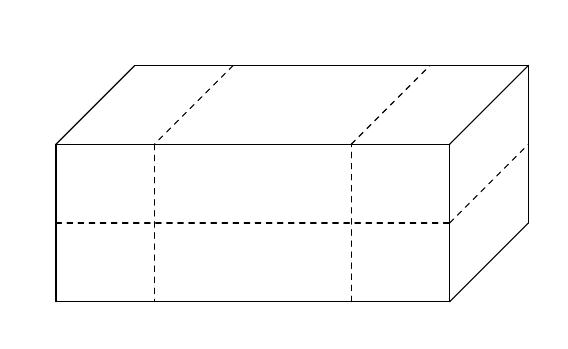
\begin{tikzpicture}[line cap=round,line join=round,>=triangle 45,x=1.0cm,y=1.0cm]
\clip(-2.3600000000000003,-0.24000000000000235) rectangle (4.139999999999999,3.479999999999999);
\draw (-2.0,2.0)-- (-2.0,0.0);
\draw (-2.0,0.0)-- (3.0,0.0);
\draw (3.0,0.0)-- (4.0,1.0);
\draw (4.0,1.0)-- (4.0,3.0);
\draw (4.0,3.0)-- (3.0,2.0);
\draw (3.0,2.0)-- (-2.0,2.0);
\draw (3.0,2.0)-- (3.0,0.0);
\draw (-2.0,2.0)-- (-1.0,3.0);
\draw (-1.0,3.0)-- (4.0,3.0);
\draw [dash pattern=on 2pt off 2pt] (0.25,3.0)-- (-0.75,2.0);
\draw [dash pattern=on 2pt off 2pt] (-0.75,2.0)-- (-0.75,0.0);
\draw [dash pattern=on 2pt off 2pt] (1.75,0.0)-- (1.75,2.0);
\draw [dash pattern=on 2pt off 2pt] (1.75,2.0)-- (2.75,3.0);
\draw [dash pattern=on 2pt off 2pt] (-2.0,1.0)-- (3.0,1.0);
\draw [dash pattern=on 2pt off 2pt] (3.0,1.0)-- (4.0,2.0);
\end{tikzpicture}
\end{center}

\noindent Hogyan válasszuk meg a méretét, hogy a legkevesebb kötöző zsinegre legyen szükségünk?
\end{enumerate}



\end{document}
